\begin{frame}
    \autotitle
    \begin{center}
        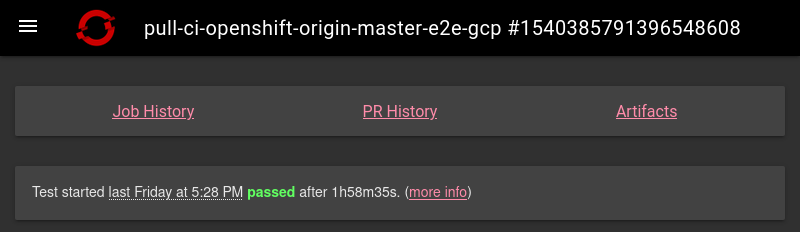
\includegraphics[width=\textwidth]{img/job.png}
        \footnotesize
        \url{https://prow.ci.openshift.org/view/gs/origin-ci-test/pr-logs/pull/27275/pull-ci-openshift-origin-master-e2e-gcp/1540385791396548608}
    \end{center}
    \note{
        From here, it is instructive to examine a typical E2E test, which
        differs quite a bit from the simple container tests we have considered
        so far.  We will look at this test in \texttt{openshift/origin} which
        creates an ephemeral GCP cluster.
    }
\end{frame}

\begin{frame}[fragile]
    \autotitle
    \footnotesize
    \url{https://github.com/openshift/release/blob/master/ci-operator/config/openshift/origin/openshift-origin-master.yaml}
    \normalsize
    \begin{verbatim}
tests:
- as: e2e-gcp
  steps:
    cluster_profile: gcp-openshift-gce-devel-ci-2
    workflow: openshift-e2e-gcp-loki
    \end{verbatim}
    \note{
        This job is generated from this innocent-looking entry in the
        \texttt{ci-operator} configuration file.

        N.b.: take it from someone who has seen all incarnations of Prow job
        definitions we have had, the fact that this test is generated from these
        four lines is a \emph{miracle}.
    }
\end{frame}

\begin{frame}[fragile]
    \autotitle
    \tiny
    \begin{verbatim}
INFO[2022-06-24T17:28:45Z] ci-operator version v20220621-3b245f722
INFO[2022-06-24T17:28:45Z] Loading configuration from https://config.ci.openshift.org for openshift/…
INFO[2022-06-24T17:28:46Z] Resolved source https://github.com/openshift/origin to master@a946e2b9, m…
INFO[2022-06-24T17:28:46Z] Building release previous from a snapshot of ocp/4.10
INFO[2022-06-24T17:28:46Z] Building release initial from a snapshot of ocp/4.11
INFO[2022-06-24T17:28:46Z] Building release latest from a snapshot of ocp/4.11
INFO[2022-06-24T17:28:47Z] Using namespace https://console.build02.ci.openshift.org/k8s/cluster/proj…
INFO[2022-06-24T17:28:47Z] Running [input:root], [input:ocp_builder_rhel-8-golang-1.15-openshift-4.8…
INFO[2022-06-24T17:28:47Z] Tagging ocp/builder:rhel-8-golang-1.15-openshift-4.8 into pipeline:ocp_bu…
INFO[2022-06-24T17:28:47Z] Tagging ocp/builder:rhel-8-golang-1.18-openshift-4.11 into pipeline:ocp_b…
…
INFO[2022-06-24T17:28:48Z] Building src
INFO[2022-06-24T17:32:03Z] Build src succeeded after 3m57s
INFO[2022-06-24T17:32:03Z] Building hello-openshift
INFO[2022-06-24T17:32:03Z] Building tests
INFO[2022-06-24T17:35:23Z] Build hello-openshift succeeded after 3m20s
INFO[2022-06-24T17:35:23Z] Tagging hello-openshift into stable
INFO[2022-06-24T17:42:13Z] Build tests succeeded after 6m48s
INFO[2022-06-24T17:42:13Z] Tagging tests into stable
INFO[2022-06-24T17:42:14Z] Creating release image registry.build02.ci.openshift.org/ci-op-8yq06grj/r…
INFO[2022-06-24T17:43:34Z] Snapshot integration stream into release 4.11.0-0.ci.test-2022-06-24-1742…
INFO[2022-06-24T17:43:34Z] Acquiring leases for test e2e-gcp: [gcp-openshift-gce-devel-ci-2-quota-sl…
INFO[2022-06-24T17:43:34Z] Acquired 1 lease(s) for gcp-openshift-gce-devel-ci-2-quota-slice: [us-cen…
INFO[2022-06-24T17:43:34Z] Running multi-stage test e2e-gcp
INFO[2022-06-24T17:43:34Z] Running multi-stage phase pre
INFO[2022-06-24T17:43:34Z] Running step e2e-gcp-ipi-install-hosted-loki.
…
INFO[2022-06-24T19:27:16Z] Releasing leases for test e2e-gcp
INFO[2022-06-24T19:27:17Z] Ran for 1h58m30s
INFO[2022-06-24T19:27:17Z] Reporting job state 'succeeded'
    \end{verbatim}
    \note{Here is what the output looks like.}
\end{frame}

\begin{frame}
    \autotitle
    \begin{center}
        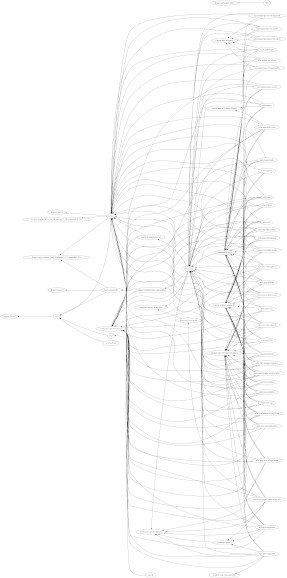
\includegraphics[scale=.35]{img/graph_origin_full.jpg} \\
    \end{center}
    \note{(a reminder that this is what we are dealing with)}
\end{frame}

\begin{frame}
    \autotitle
    \begin{center}
        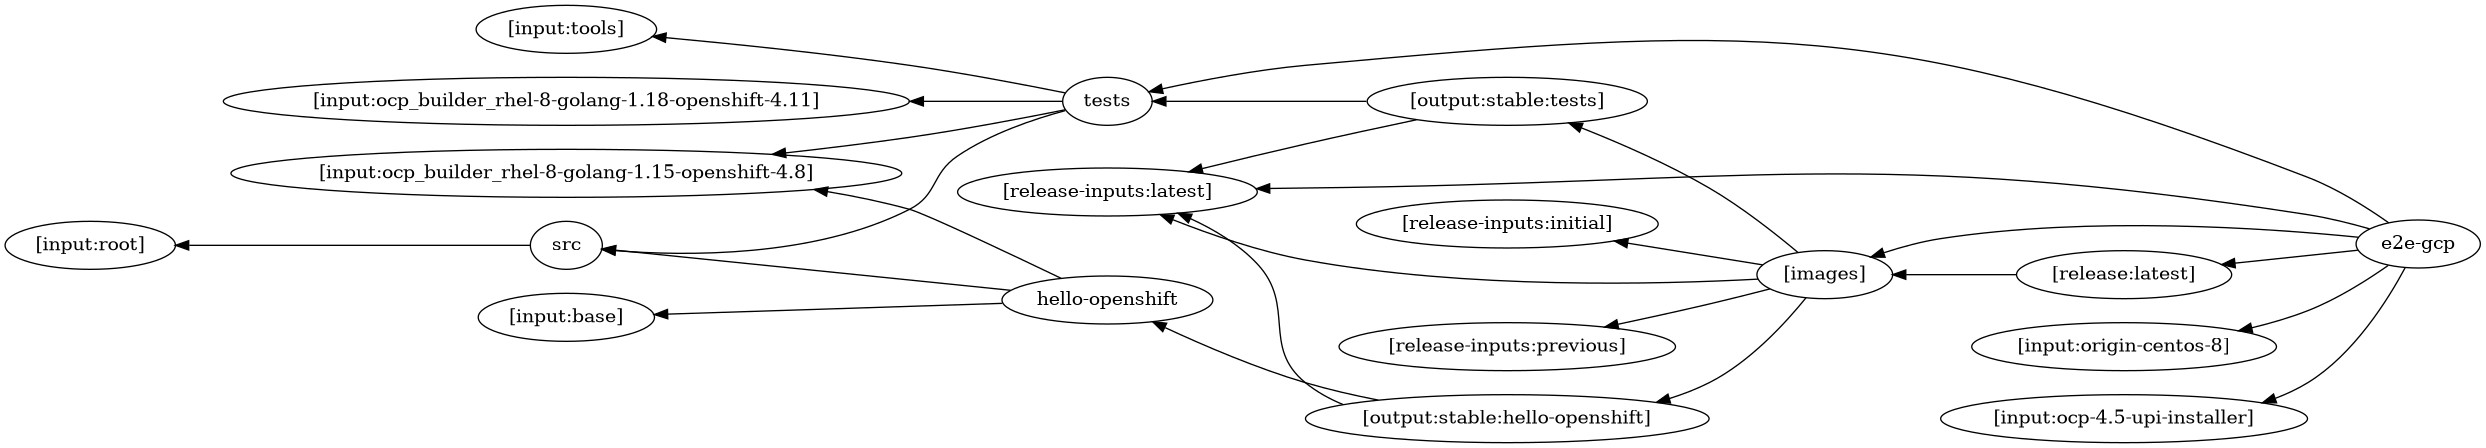
\includegraphics[width=\textwidth]{img/graph_origin_gcp.jpg} \\
    \end{center}
    \note{
        Thankfully, for this particular test, we "only" have to deal with this
        sub-graph.  Let's examine each part.
    }
\end{frame}

\begin{frame}[fragile]
    \autotitle
    \small
    \begin{verbatim}
ci-operator version v20220621-3b245f722
Loading configuration \
    from https://config.ci.openshift.org \
    for openshift/origin@master
Resolved source https://github.com/openshift/origin \
    to master@a946e2b9, merging: \
    #27275 457391d6 @DennisPeriquet
    \end{verbatim}
    \note{We start with the part you are already familiar with.}
\end{frame}

\begin{frame}[fragile]
    \autotitle
    \small
    \begin{verbatim}
Building release previous from a snapshot of ocp/4.10
Building release initial from a snapshot of ocp/4.11
Building release latest from a snapshot of ocp/4.11
    \end{verbatim}
    \footnotesize
    \begin{verbatim}
releases:
  initial:
    integration:
      name: "4.11"
      namespace: ocp
  latest:
    integration:
      include_built_images: true
      name: "4.11"
      namespace: ocp
  previous:
    integration:
      name: "4.10"
      namespace: ocp
    \end{verbatim}
    \note{
        Release images are also root nodes, so they are imported immediately.
        These are all integration streams, which means they come from an
        \texttt{ImageStream} and can simply be copied into the test namespace
        (this is what "snapshot" refers to).
    }
\end{frame}

\begin{frame}
    \autotitle
    \begin{center}
        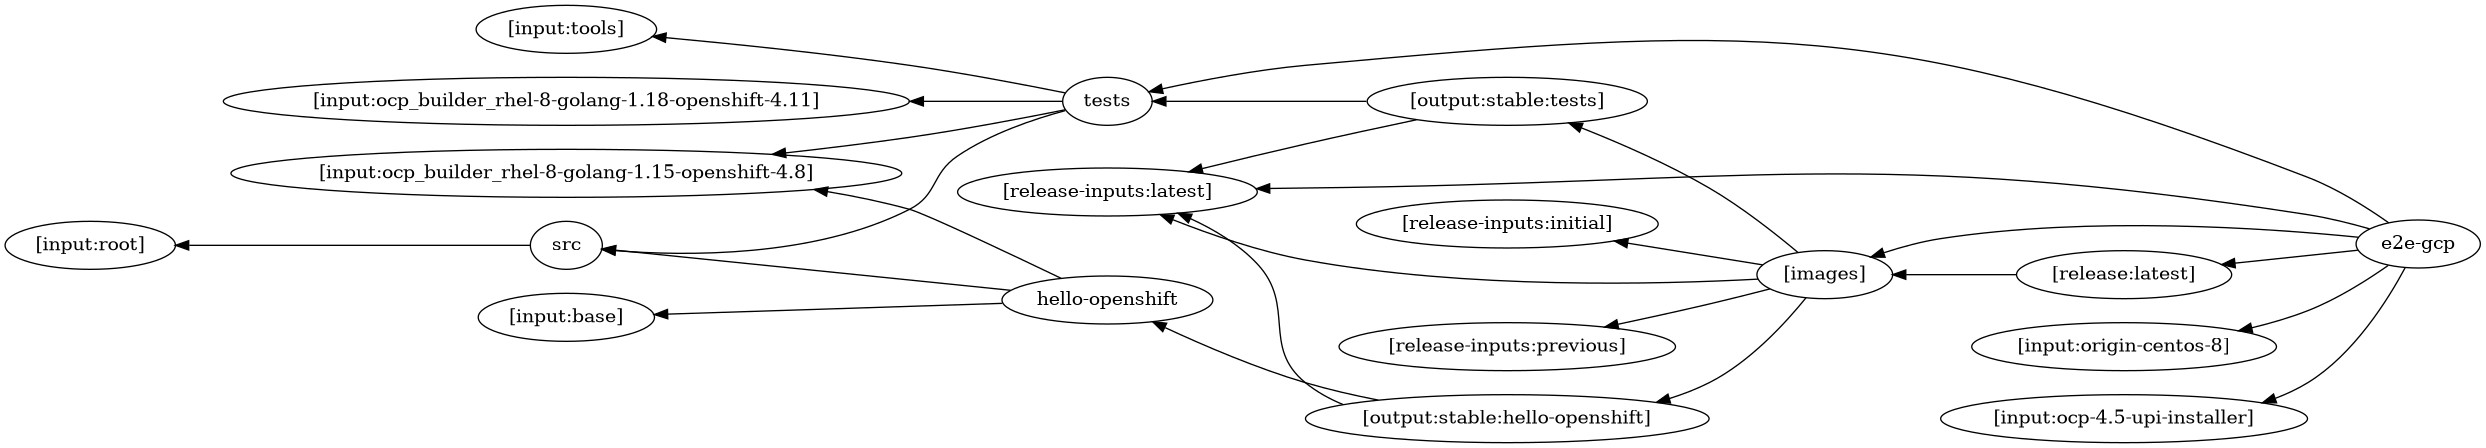
\includegraphics
            [width=\textwidth, clip, trim=900bp 0 700bp 0]
            {img/graph_origin_gcp.jpg}
    \end{center}
    \note{These correspond to the \texttt{[release-inputs:…]} steps here.}
\end{frame}

\begin{frame}[fragile]
    \autotitle
    \footnotesize
    \begin{verbatim}
Using namespace https://console.build02.ci.openshift.org/\
    k8s/cluster/projects/ci-op-8yq06grj
Running [input:root], \
    [input:ocp_builder_rhel-8-golang-1.15-openshift-4.8], \
    [input:ocp_builder_rhel-8-golang-1.18-openshift-4.11], \
    [input:tools], [input:base], [input:origin-centos-8], \
    [input:ocp-4.5-upi-installer], [release-inputs:previous], \
    [release-inputs:initial], [release-inputs:latest], \
    src, tests, hello-openshift, \
    [output:stable:tests], [output:stable:hello-openshift], \
    [images], [release:latest], e2e-gcp
    \end{verbatim}
    \note{
        Here we get assigned a temporary namespace and print the execution
        graph.  Note the same left-to-right order of dependencies, with the
        actual test at the far right of the list.
    }
\end{frame}

\begin{frame}[fragile]
    \autotitle
    \scriptsize
    \begin{verbatim}
Tagging ocp/builder:rhel-8-golang-1.15-openshift-4.8 into \
    pipeline:ocp_builder_rhel-8-golang-1.15-openshift-4.8.
Tagging ocp/builder:rhel-8-golang-1.18-openshift-4.11 into \
    pipeline:ocp_builder_rhel-8-golang-1.18-openshift-4.11.
Tagging openshift/release:rhel-8-release-golang-1.18-openshift-4.11 \
    into pipeline:root.
Tagging origin/centos:8 into pipeline:origin-centos-8.
Tagging ocp/4.11:base into pipeline:base.
Tagging ocp/4.5:upi-installer into pipeline:ocp-4.5-upi-installer.
Tagging ocp/4.11:tools into pipeline:tools.
    \end{verbatim}
    \note{
        The roots of the graph are usually input images, since both the build
        root and base images are depended on for image builds and tests.
    }
\end{frame}

\begin{frame}
    \autotitle
    \begin{center}
        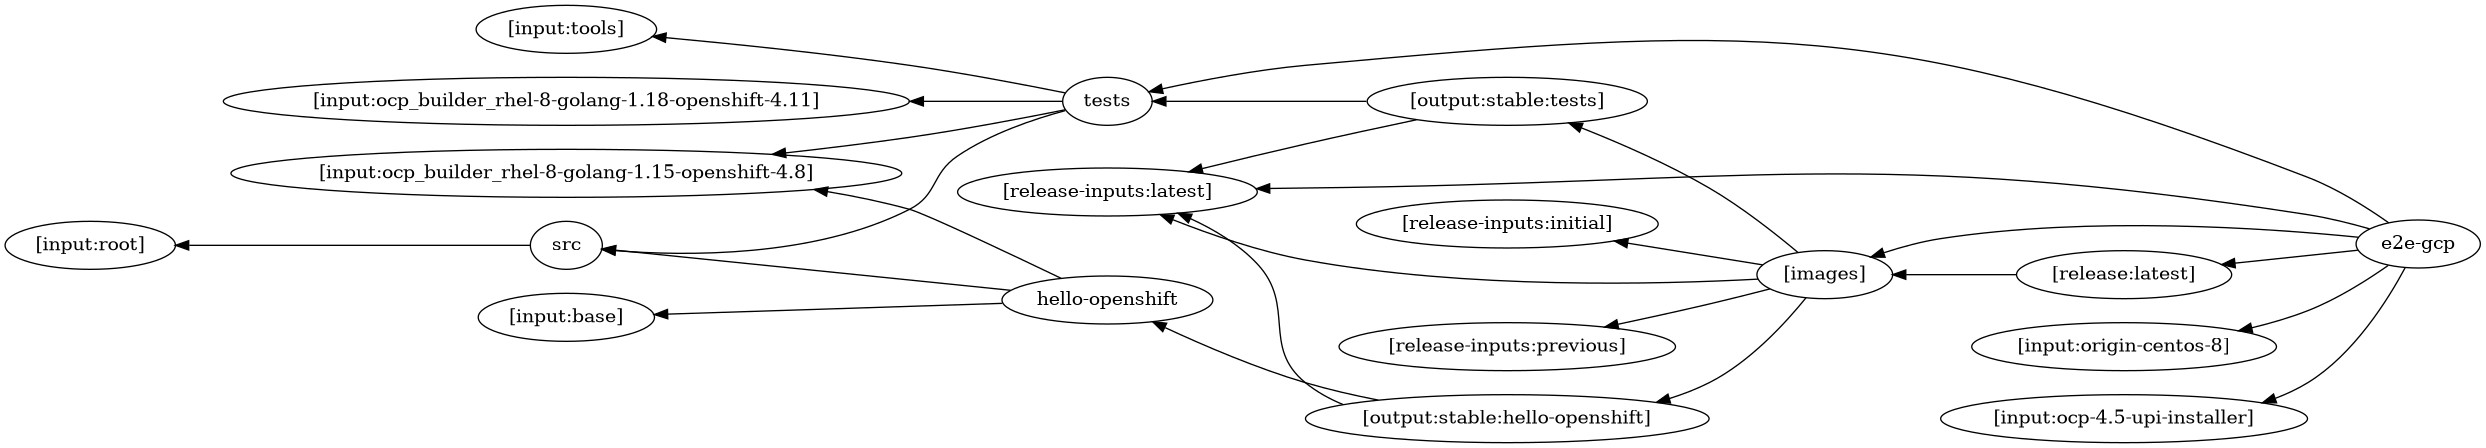
\includegraphics
            [width=\textwidth, clip, trim=0 0 1300bp 0]
            {img/graph_origin_gcp.jpg}
    \end{center}
    \note{
        We see them at the far left side of the graph: they are all in the
        format \texttt{[input:…]}.  Note the dependent image builds.
    }
\end{frame}

\begin{frame}
    \autotitle
    \begin{center}
        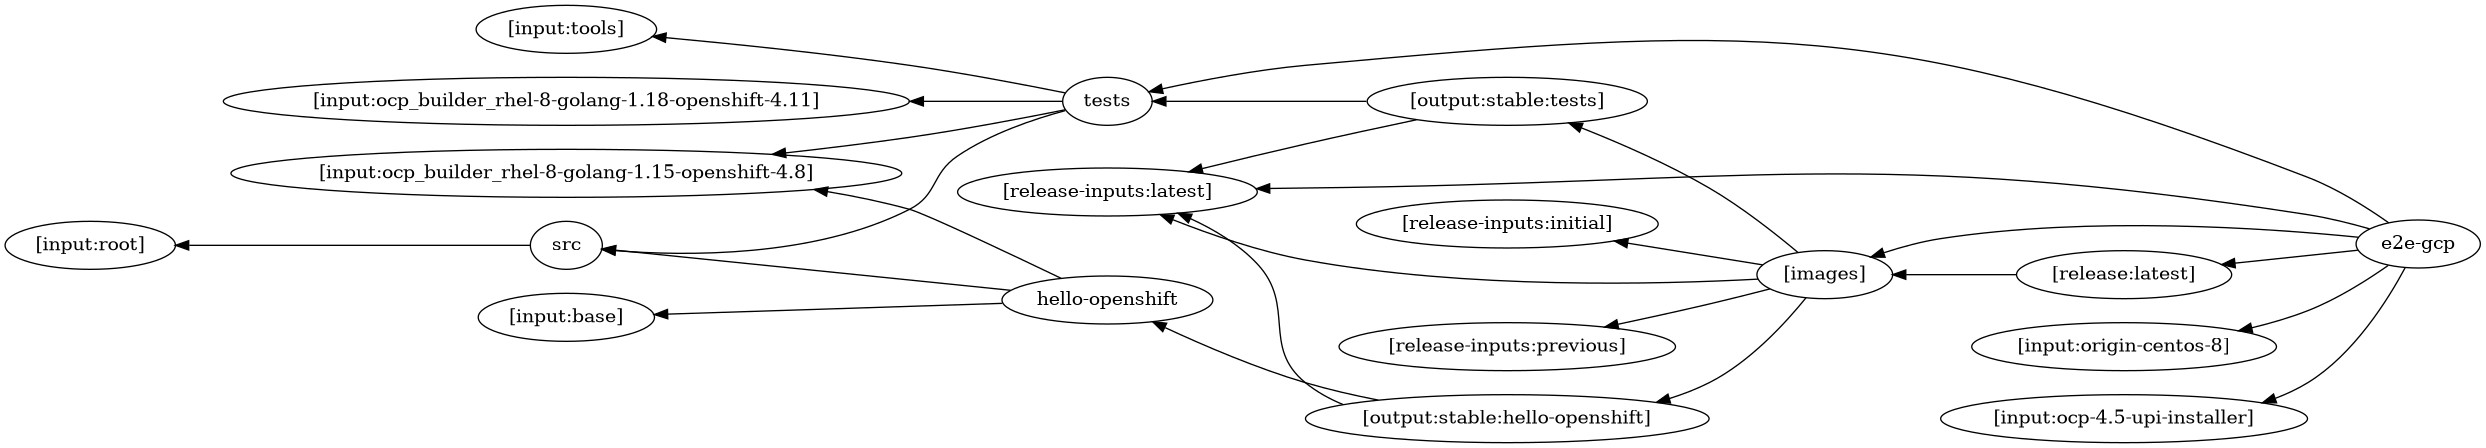
\includegraphics
            [scale=.4, clip, trim=1900bp 0 0 0]
            {img/graph_origin_gcp.jpg}
    \end{center}
    \note{
        And again at the far right for input images depended on by the test
        (more on that later).  These are all independent, so they are imported
        in parallel.
    }
\end{frame}

\begin{frame}[fragile]
    \autotitle
    \footnotesize
    \begin{verbatim}
base_images:
  base: {…}
  ocp_builder_rhel-8-golang-1.15-openshift-4.8: {…}
  ocp_builder_rhel-8-golang-1.18-openshift-4.11: {…}
  tools: {…}
    \end{verbatim}
    \note{
        These images are imported directly using \texttt{base\_images}.
    }
\end{frame}

\begin{frame}[fragile]
    \autotitle
    \begin{verbatim}
build_root:
  from_repository: true
    \end{verbatim}
    \small
    \url{https://github.com/openshift/origin/blob/master/.ci-operator.yaml}
    \normalsize
    \begin{verbatim}
build_root_image:
  name: release
  namespace: openshift
  tag: rhel-8-release-golang-1.18-openshift-4.11
    \end{verbatim}
    \note{
        The \texttt{build\_root} image comes from the repository (you can see
        how these things start to get difficult to track).

        As an aside, when \texttt{from\_repository} is used, we have to make
        sure the Prow job (which executes \texttt{ci-operator}) is configured
        with \texttt{decorate} and does not have \texttt{skip\_cloning}.
        \texttt{ci-operator} will then have access to the the repository code,
        where the \texttt{.ci-operator.yaml} file resides.
    }
\end{frame}

\begin{frame}[fragile]
    \autotitle
    \footnotesize
    \url{https://steps.ci.openshift.org/workflow/openshift-e2e-gcp-loki}
    \small
    \begin{verbatim}
workflow:
  as: openshift-e2e-gcp-loki
  steps:
    allow_best_effort_post_steps: true
    pre:
    - ref: ipi-install-hosted-loki
    - chain: ipi-gcp-pre
    test:
    - ref: openshift-e2e-test
    post:
    - chain: ipi-gcp-post
  documentation: |-
    The Openshift E2E GCP workflow executes the common
    end-to-end test suite on GCP with a default cluster
    configuration with loki as log collector.
    \end{verbatim}
    \note{
        Finding the source of the other images requires us to start looking into
        multi-stage tests.  The \texttt{openshift-e2e-gcp-loki} workflow
        declared in the test can be found in the step registry.  It includes a
        chain called \texttt{ipi-gcp-pre}…
    }
\end{frame}

\begin{frame}[fragile]
    \autotitle
    \url{https://steps.ci.openshift.org/chain/ipi-gcp-pre}
    \begin{verbatim}
chain:
  as: ipi-gcp-pre
  steps:
  - chain: ipi-conf-gcp
  - chain: ipi-install
  documentation: |-
    The IPI setup step contains all steps that
    provision an OpenShift cluster with a default
    configuration on GCP.
    \end{verbatim}
    \note{which includes a chain called \texttt{ipi-conf-gcp}…}
\end{frame}

\begin{frame}[fragile]
    \autotitle
    \url{https://steps.ci.openshift.org/chain/ipi-conf-gcp}
    \begin{verbatim}
chain:
  as: ipi-conf-gcp
  steps:
  - ref: ipi-conf
  - ref: ipi-conf-gcp
  - ref: ipi-install-monitoringpvc
  documentation: >-
    This chain generates an install-config.yaml
    file configured to run clusters in the GCP CI
    project.
    The GCP specific configs are added to
    the file generated by the ipi-conf steps.
    This resulting file is stored in the shared
    directory for future consumption.
    \end{verbatim}
    \note{
        which includes steps called \texttt{ipi-conf} and \texttt{ipi-conf-gcp}…
    }
\end{frame}

\begin{frame}[fragile]
    \autotitle
    \small
    \url{https://steps.ci.openshift.org/reference/ipi-conf}
    \url{https://steps.ci.openshift.org/reference/ipi-conf-gcp}
    \normalsize
    \begin{verbatim}
ref:
  as: ipi-conf
  from_image:
   namespace: origin
   name: centos
   tag: '8'
    \end{verbatim}
    ($\texttt{from\_image} \approx \texttt{base\_images} + \texttt{from}$)
    \note{
        and here we finally find our \texttt{centos:8} image.
        \texttt{from\_image} entries for all steps are collected and added to
        the input images in \texttt{base\_images}.
    }
\end{frame}

\begin{frame}[fragile]
    \autotitle
    \footnotesize
    \url{https://steps.ci.openshift.org/reference/gather-gcp-console}
    \normalsize
    \begin{verbatim}
ref:
  as: gather-gcp-console
  optional_on_success: true
  from_image:
    namespace: ocp
    name: "4.5"
    tag: upi-installer
    …
    \end{verbatim}
    \note{
        Similarly, \texttt{upi-installer} can be found in the
        \texttt{gather-gcp-console} step.
    }
\end{frame}

\begin{frame}[fragile]
    \autotitle
    \small
    \begin{verbatim}
Building src
Build src succeeded after 3m57s
Building hello-openshift
Building tests
Build hello-openshift succeeded after 3m20s
Tagging hello-openshift into stable
Build tests succeeded after 6m48s
Tagging tests into stable
    \end{verbatim}
    \note{
        After the required images are imported, image builds can be started.
    }
\end{frame}

\begin{frame}
    \autotitle
    \begin{center}
        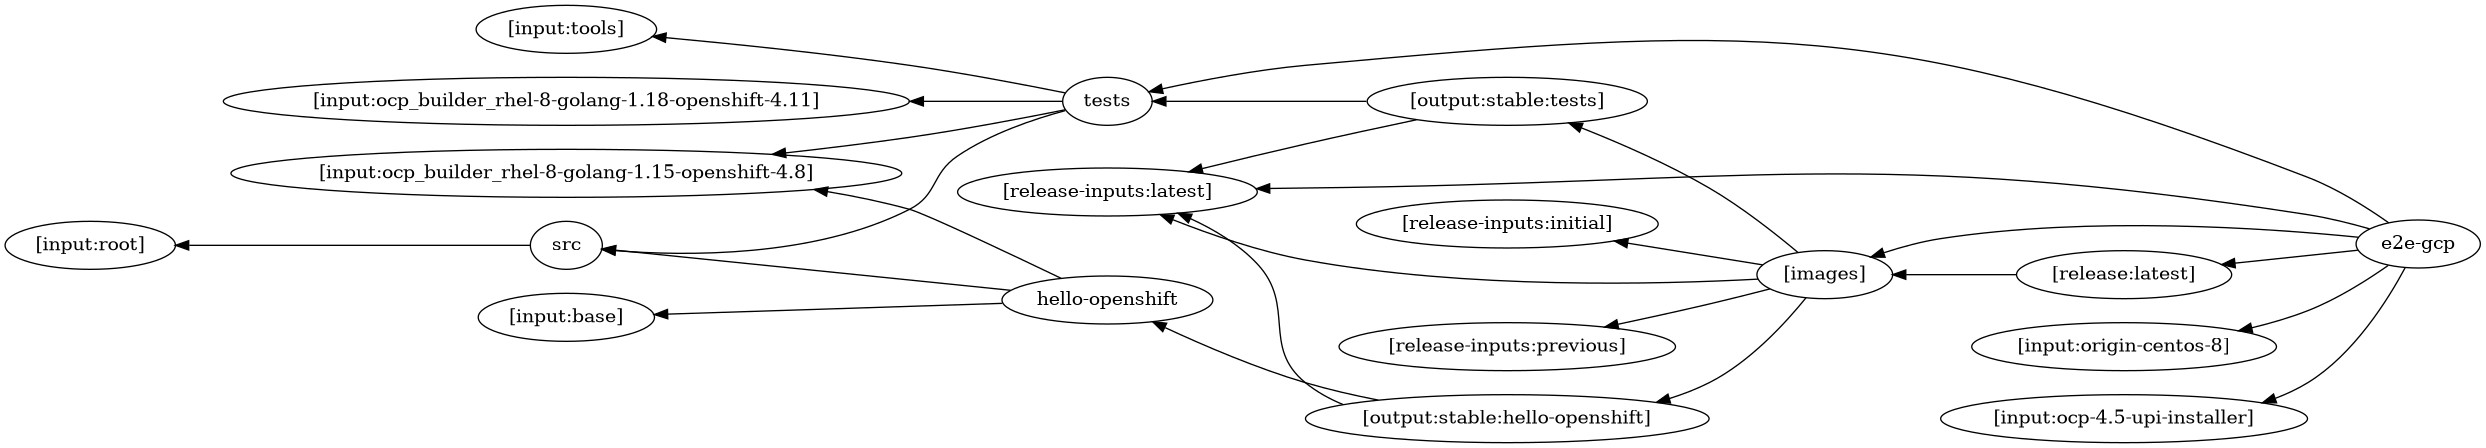
\includegraphics
            [width=\textwidth, clip, trim=450bp 0 1200bp 0]
            {img/graph_origin_gcp.jpg}
    \end{center}
    \note{
        \texttt{src} is built first, since it is a requirement for the other
        two, which are then built in parallel.
    }
\end{frame}

\begin{frame}[fragile]
    \autotitle
    \small
    \begin{verbatim}
Build hello-openshift succeeded after 3m20s
Tagging hello-openshift into stable
Build tests succeeded after 6m48s
Tagging tests into stable
    \end{verbatim}
    \note{
        Each image that is built is also tagged into the \texttt{stable}
        \texttt{ImageStream}.
    }
\end{frame}

\begin{frame}
    \autotitle
    \begin{center}
        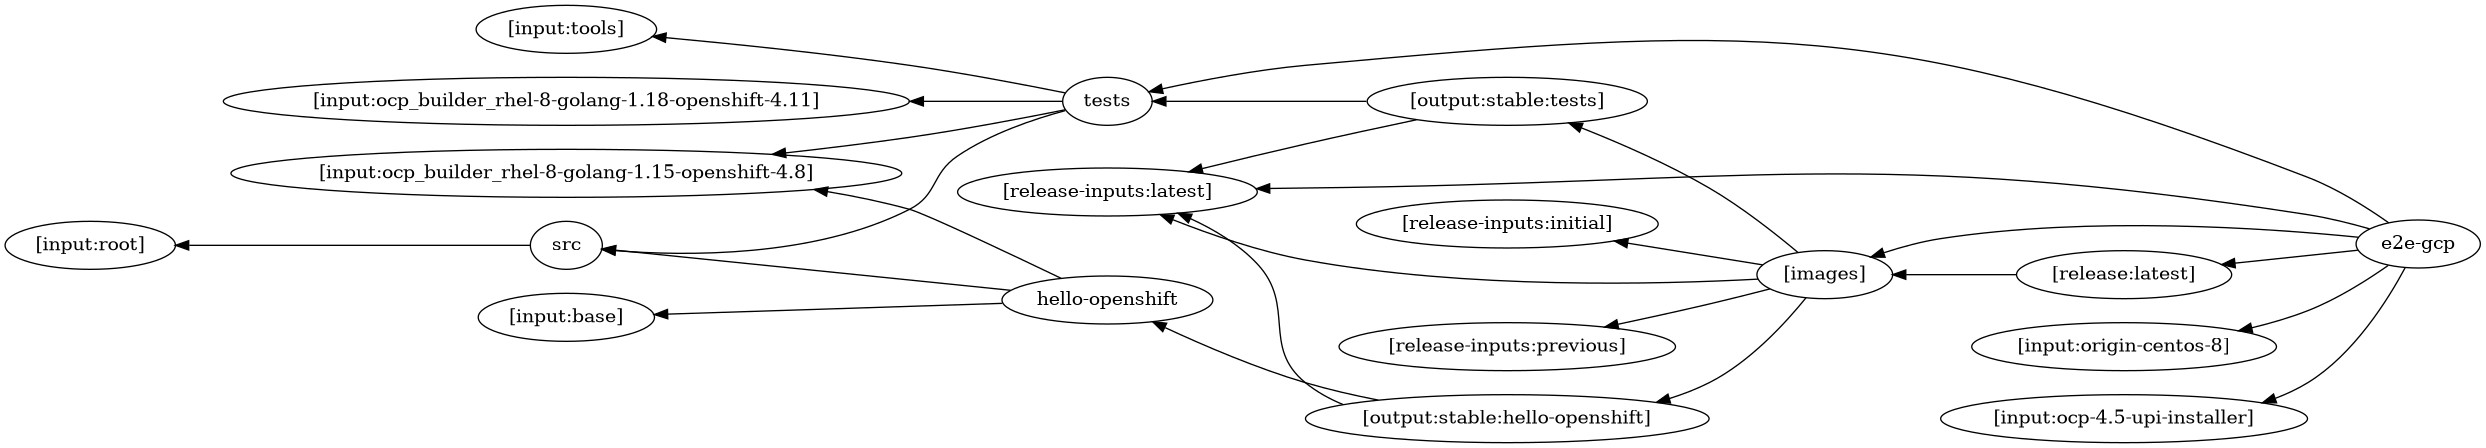
\includegraphics
            [width=\textwidth, clip, trim=950bp 0 550bp 0]
            {img/graph_origin_gcp.jpg}
    \end{center}
    \note{These are done by the steps in the format \texttt{[output:…]}.}
\end{frame}

\begin{frame}
    \autotitle
    \begin{center}
        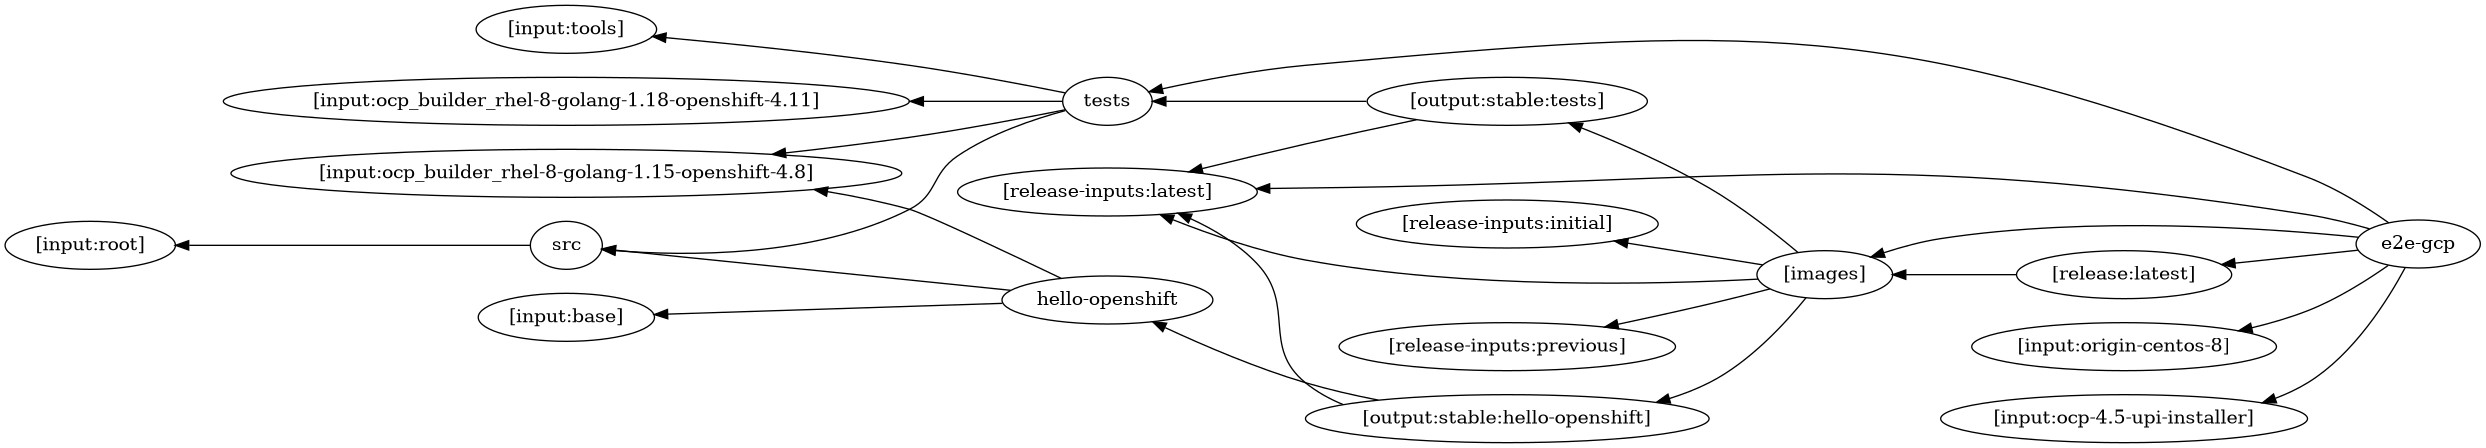
\includegraphics
            [width=\textwidth, clip, trim=950bp 0 0 0]
            {img/graph_origin_gcp.jpg}
    \end{center}
    \note{
        This is difficult to capture since it is right in the middle of the
        graph, but notice the \texttt{[images]} step acting as a synchronization
        point between image build / release image imports and the release
        payload generation / test.

        That is all it does: it is a synthetic step created purely to guarantee
        these operations are done in the proper order.
    }
\end{frame}

\begin{frame}[fragile]
    \autotitle
    \footnotesize
    \url{https://github.com/openshift/release/blob/master/ci-operator/jobs/openshift/origin/openshift-origin-master-postsubmits.yaml}
    (simplified)
    \normalsize
    \begin{verbatim}
name: branch-ci-openshift-origin-master-images
spec:
  containers:
  - args:
    - --target=[images]
    - --promote
    command:
    - ci-operator
    \end{verbatim}
    \note{
        It can also be used as a target, such as we do in the \texttt{*-images}
        post-submit jobs.
    }
\end{frame}

\begin{frame}[fragile]
    \autotitle
    \footnotesize
    \begin{verbatim}
Creating release image registry.build02.ci.openshift.org/\
    ci-op-8yq06grj/release:latest.
Snapshot integration stream into release \
    4.11.0-0.ci.test-2022-06-24-174214-ci-op-8yq06grj-latest \
    to tag release:latest
    \end{verbatim}
    \note{
        We now create the release payload from the \texttt{stable}
        \texttt{ImageStream}.  The latter contains the initial images imported
        from the integration stream, along with the images just built from the
        input source code (recall they were tagged into \texttt{stable} after
        they were built).

        By overlaying the new tags on top of the existing streams, we get a
        release payload where the repository images are overwritten by the ones
        which were just built from the input source code.
    }
\end{frame}

\begin{frame}[fragile]
    \autotitle
    \begin{verbatim}
releases:
  latest:
    integration:
      include_built_images: true
      name: "4.11"
      namespace: ocp
    \end{verbatim}
\end{frame}

\begin{frame}
    \autotitle
    \begin{center}
        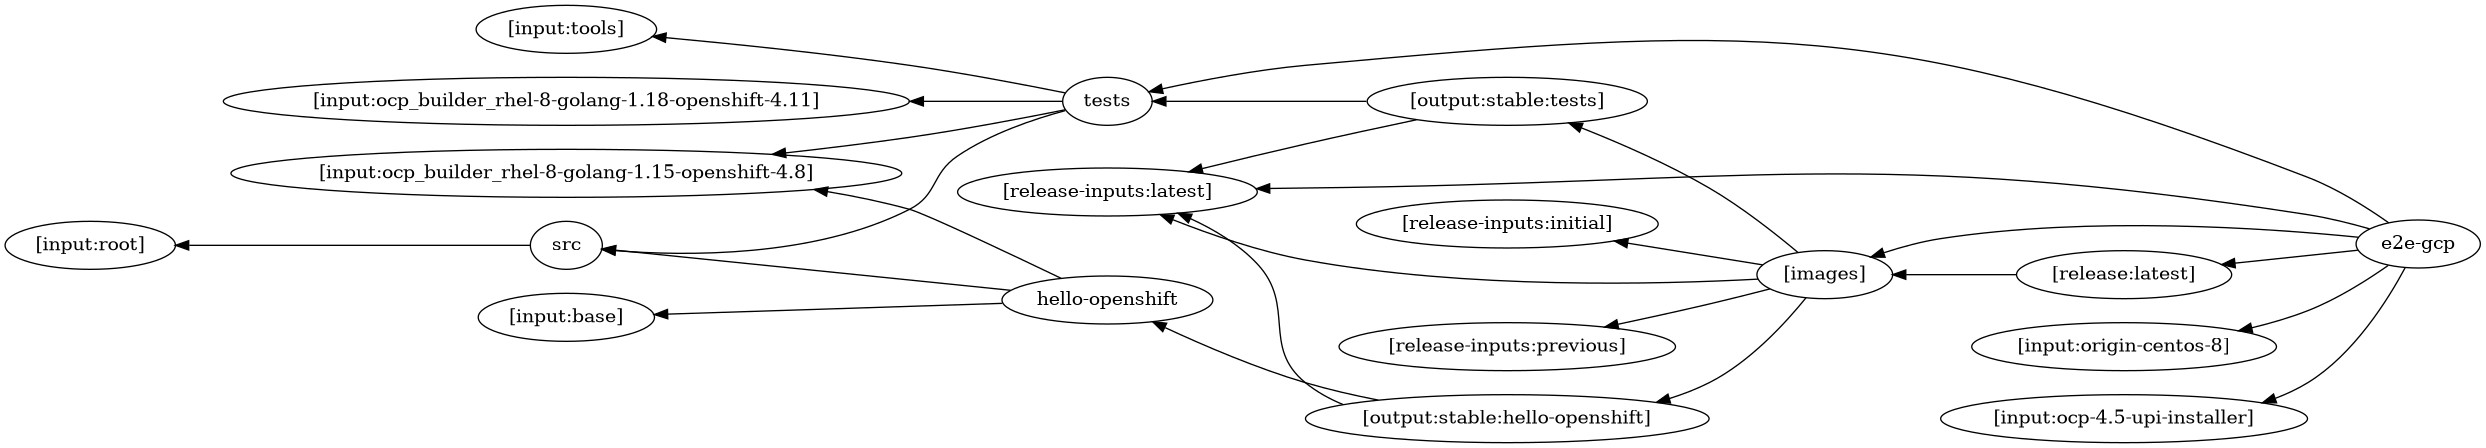
\includegraphics
            [width=\textwidth, clip, trim=1600bp 0 100bp 0]
            {img/graph_origin_gcp.jpg}
    \end{center}
    \note{
        This is what the \texttt{[release:latest]} job does.  The dependency on
        that step by the E2E test makes the resulting image available to the
        latter to be used by the installer to create the ephemeral cluster.
    }
\end{frame}

\begin{frame}[fragile]
    \autotitle
    \footnotesize
    \begin{verbatim}
Acquiring leases for test e2e-gcp: \
    [gcp-openshift-gce-devel-ci-2-quota-slice]
Acquired 1 lease(s) for \
    gcp-openshift-gce-devel-ci-2-quota-slice: \
    [us-central1--gcp-openshift-gce-devel-ci-2-quota-slice-08]
    \end{verbatim}
    \note{
        We are finally at the beginning of the test execution now.  Because it
        is an E2E test (approximated by "it declares a cluster profile"),
        \texttt{ci-operator} will contact the leasing server (i.e.
        \href{https://github.com/kubernetes-sigs/boskos.git}{Boskos}) to acquire
        a lease for the ephemeral cluster.
    }
\end{frame}

\begin{frame}[fragile]
    \autotitle
    \url{https://github.com/openshift/ci-tools/blob/master/pkg/api/types.go}
    (heavily abbreviated)
    \footnotesize
    \begin{verbatim}
type ClusterProfile string

const ClusterProfileGCP2 ClusterProfile =
    "gcp-openshift-gce-devel-ci-2"

func (p ClusterProfile) LeaseType() string {
    switch p {
    case ClusterProfileGCP2:
        return "gcp-openshift-gce-devel-ci-2-quota-slice"
    }
}
    \end{verbatim}
    \note{
        Each cluster profile (a string) is registered in \texttt{ci-tools} and
        associated with a resource type.
    }
\end{frame}

\begin{frame}[fragile]
    \autotitle
    \footnotesize
    \begin{verbatim}
Running multi-stage test e2e-gcp
Running multi-stage phase pre
Running step e2e-gcp-ipi-install-hosted-loki.
Step e2e-gcp-ipi-install-hosted-loki succeeded after 20s.
Running step e2e-gcp-ipi-conf.
Step e2e-gcp-ipi-conf succeeded after 20s.
…
Running multi-stage phase test
Running step e2e-gcp-openshift-e2e-test.
Step e2e-gcp-openshift-e2e-test succeeded after 55m0s.
Step phase test succeeded after 55m0s.
Running multi-stage phase post
Running step e2e-gcp-gather-gcp-console.
Step e2e-gcp-gather-gcp-console succeeded after 50s.
…
Step phase post succeeded after 16m40s.
    \end{verbatim}
\end{frame}

\begin{frame}[fragile]
    \autotitle
    \begin{verbatim}
Releasing leases for test e2e-gcp
Ran for 1h58m30s
Reporting job state 'succeeded'
    \end{verbatim}
\end{frame}
